% Created by tikzDevice version 0.10.1 on 2018-02-09 14:59:34
% !TEX encoding = UTF-8 Unicode
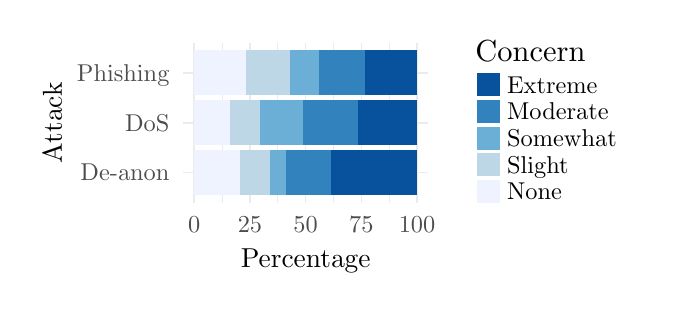
\begin{tikzpicture}[x=1pt,y=1pt]
\definecolor{fillColor}{RGB}{255,255,255}
\path[use as bounding box,fill=fillColor,fill opacity=0.00] (0,0) rectangle (224.04, 93.95);
\begin{scope}
\path[clip] ( 56.18, 30.77) rectangle (144.74, 88.45);
\definecolor{drawColor}{gray}{0.92}

\path[draw=drawColor,line width= 0.3pt,line join=round] ( 70.26, 30.77) --
	( 70.26, 88.45);

\path[draw=drawColor,line width= 0.3pt,line join=round] ( 90.39, 30.77) --
	( 90.39, 88.45);

\path[draw=drawColor,line width= 0.3pt,line join=round] (110.52, 30.77) --
	(110.52, 88.45);

\path[draw=drawColor,line width= 0.3pt,line join=round] (130.64, 30.77) --
	(130.64, 88.45);

\path[draw=drawColor,line width= 0.6pt,line join=round] ( 56.18, 41.59) --
	(144.74, 41.59);

\path[draw=drawColor,line width= 0.6pt,line join=round] ( 56.18, 59.61) --
	(144.74, 59.61);

\path[draw=drawColor,line width= 0.6pt,line join=round] ( 56.18, 77.64) --
	(144.74, 77.64);

\path[draw=drawColor,line width= 0.6pt,line join=round] ( 60.20, 30.77) --
	( 60.20, 88.45);

\path[draw=drawColor,line width= 0.6pt,line join=round] ( 80.33, 30.77) --
	( 80.33, 88.45);

\path[draw=drawColor,line width= 0.6pt,line join=round] (100.45, 30.77) --
	(100.45, 88.45);

\path[draw=drawColor,line width= 0.6pt,line join=round] (120.58, 30.77) --
	(120.58, 88.45);

\path[draw=drawColor,line width= 0.6pt,line join=round] (140.71, 30.77) --
	(140.71, 88.45);
\definecolor{fillColor}{RGB}{239,243,255}

\path[fill=fillColor] ( 60.20, 33.48) rectangle ( 76.78, 49.70);
\definecolor{fillColor}{RGB}{189,215,231}

\path[fill=fillColor] ( 76.78, 33.48) rectangle ( 87.44, 49.70);
\definecolor{fillColor}{RGB}{107,174,214}

\path[fill=fillColor] ( 87.44, 33.48) rectangle ( 93.35, 49.70);
\definecolor{fillColor}{RGB}{49,130,189}

\path[fill=fillColor] ( 93.35, 33.48) rectangle (109.54, 49.70);
\definecolor{fillColor}{RGB}{8,81,156}

\path[fill=fillColor] (109.54, 33.48) rectangle (140.72, 49.70);
\definecolor{fillColor}{RGB}{239,243,255}

\path[fill=fillColor] ( 60.20, 51.50) rectangle ( 73.16, 67.72);
\definecolor{fillColor}{RGB}{189,215,231}

\path[fill=fillColor] ( 73.16, 51.50) rectangle ( 83.77, 67.72);
\definecolor{fillColor}{RGB}{107,174,214}

\path[fill=fillColor] ( 83.77, 51.50) rectangle ( 99.47, 67.72);
\definecolor{fillColor}{RGB}{49,130,189}

\path[fill=fillColor] ( 99.47, 51.50) rectangle (119.50, 67.72);
\definecolor{fillColor}{RGB}{8,81,156}

\path[fill=fillColor] (119.50, 51.50) rectangle (140.71, 67.72);
\definecolor{fillColor}{RGB}{239,243,255}

\path[fill=fillColor] ( 60.20, 69.53) rectangle ( 79.05, 85.75);
\definecolor{fillColor}{RGB}{189,215,231}

\path[fill=fillColor] ( 79.05, 69.53) rectangle ( 94.75, 85.75);
\definecolor{fillColor}{RGB}{107,174,214}

\path[fill=fillColor] ( 94.75, 69.53) rectangle (105.36, 85.75);
\definecolor{fillColor}{RGB}{49,130,189}

\path[fill=fillColor] (105.36, 69.53) rectangle (121.85, 85.75);
\definecolor{fillColor}{RGB}{8,81,156}

\path[fill=fillColor] (121.85, 69.53) rectangle (140.70, 85.75);
\end{scope}
\begin{scope}
\path[clip] (  0.00,  0.00) rectangle (224.04, 93.95);
\definecolor{drawColor}{gray}{0.30}

\node[text=drawColor,anchor=base east,inner sep=0pt, outer sep=0pt, scale=  0.88] at ( 51.23, 38.56) {De-anon};

\node[text=drawColor,anchor=base east,inner sep=0pt, outer sep=0pt, scale=  0.88] at ( 51.23, 56.58) {DoS};

\node[text=drawColor,anchor=base east,inner sep=0pt, outer sep=0pt, scale=  0.88] at ( 51.23, 74.61) {Phishing};
\end{scope}
\begin{scope}
\path[clip] (  0.00,  0.00) rectangle (224.04, 93.95);
\definecolor{drawColor}{gray}{0.30}

\node[text=drawColor,anchor=base,inner sep=0pt, outer sep=0pt, scale=  0.88] at ( 60.20, 19.76) {0};

\node[text=drawColor,anchor=base,inner sep=0pt, outer sep=0pt, scale=  0.88] at ( 80.33, 19.76) {25};

\node[text=drawColor,anchor=base,inner sep=0pt, outer sep=0pt, scale=  0.88] at (100.45, 19.76) {50};

\node[text=drawColor,anchor=base,inner sep=0pt, outer sep=0pt, scale=  0.88] at (120.58, 19.76) {75};

\node[text=drawColor,anchor=base,inner sep=0pt, outer sep=0pt, scale=  0.88] at (140.71, 19.76) {100};
\end{scope}
\begin{scope}
\path[clip] (  0.00,  0.00) rectangle (224.04, 93.95);
\definecolor{drawColor}{RGB}{0,0,0}

\node[text=drawColor,anchor=base,inner sep=0pt, outer sep=0pt, scale=  0.99] at (100.46,  7.44) {Percentage};
\end{scope}
\begin{scope}
\path[clip] (  0.00,  0.00) rectangle (224.04, 93.95);
\definecolor{drawColor}{RGB}{0,0,0}

\node[text=drawColor,rotate= 90.00,anchor=base,inner sep=0pt, outer sep=0pt, scale=  0.99] at ( 12.32, 59.61) {Attack};
\end{scope}
\begin{scope}
\path[clip] (  0.00,  0.00) rectangle (224.04, 93.95);
\definecolor{drawColor}{RGB}{0,0,0}

\node[text=drawColor,anchor=base west,inner sep=0pt, outer sep=0pt, scale=  1.10] at (161.81, 81.72) {Concern};
\end{scope}
\begin{scope}
\path[clip] (  0.00,  0.00) rectangle (224.04, 93.95);
\definecolor{fillColor}{RGB}{8,81,156}

\path[fill=fillColor] (162.52, 69.18) rectangle (170.74, 77.40);
\end{scope}
\begin{scope}
\path[clip] (  0.00,  0.00) rectangle (224.04, 93.95);
\definecolor{fillColor}{RGB}{49,130,189}

\path[fill=fillColor] (162.52, 59.55) rectangle (170.74, 67.76);
\end{scope}
\begin{scope}
\path[clip] (  0.00,  0.00) rectangle (224.04, 93.95);
\definecolor{fillColor}{RGB}{107,174,214}

\path[fill=fillColor] (162.52, 49.91) rectangle (170.74, 58.12);
\end{scope}
\begin{scope}
\path[clip] (  0.00,  0.00) rectangle (224.04, 93.95);
\definecolor{fillColor}{RGB}{189,215,231}

\path[fill=fillColor] (162.52, 40.27) rectangle (170.74, 48.49);
\end{scope}
\begin{scope}
\path[clip] (  0.00,  0.00) rectangle (224.04, 93.95);
\definecolor{fillColor}{RGB}{239,243,255}

\path[fill=fillColor] (162.52, 30.64) rectangle (170.74, 38.85);
\end{scope}
\begin{scope}
\path[clip] (  0.00,  0.00) rectangle (224.04, 93.95);
\definecolor{drawColor}{RGB}{0,0,0}

\node[text=drawColor,anchor=base west,inner sep=0pt, outer sep=0pt, scale=  0.88] at (173.26, 70.26) {Extreme};
\end{scope}
\begin{scope}
\path[clip] (  0.00,  0.00) rectangle (224.04, 93.95);
\definecolor{drawColor}{RGB}{0,0,0}

\node[text=drawColor,anchor=base west,inner sep=0pt, outer sep=0pt, scale=  0.88] at (173.26, 60.62) {Moderate};
\end{scope}
\begin{scope}
\path[clip] (  0.00,  0.00) rectangle (224.04, 93.95);
\definecolor{drawColor}{RGB}{0,0,0}

\node[text=drawColor,anchor=base west,inner sep=0pt, outer sep=0pt, scale=  0.88] at (173.26, 50.99) {Somewhat};
\end{scope}
\begin{scope}
\path[clip] (  0.00,  0.00) rectangle (224.04, 93.95);
\definecolor{drawColor}{RGB}{0,0,0}

\node[text=drawColor,anchor=base west,inner sep=0pt, outer sep=0pt, scale=  0.88] at (173.26, 41.35) {Slight};
\end{scope}
\begin{scope}
\path[clip] (  0.00,  0.00) rectangle (224.04, 93.95);
\definecolor{drawColor}{RGB}{0,0,0}

\node[text=drawColor,anchor=base west,inner sep=0pt, outer sep=0pt, scale=  0.88] at (173.26, 31.71) {None};
\end{scope}
\end{tikzpicture}
